\chapter{Background and Related Work}
\label{chapter:background}

\section{Computational Fluid Dynamics}
\label{sec:cfd}

Before simulating fluid flows, one has to mathematically model them. The choice of model mostly depends on the scale of the flow and the properties of the fluid.

The vast majority of CFD simulations are for macroscopic flows where the fluid can be treated as a continuum.
Fluid flows modeled as a continuum are usually modeled by partial differential equations, most notable of which being the \emph{Navier-Stokes Equations}. The equations take different forms depending on the specific properties of the fluid, such as compressibility, viscosity or heat transfer.
For example, the momentum equation written in conservation form for an incompressible fluid is:
\begin{displaymath}
    \label{eq:ns}
    \frac{\partial}{\partial t} \rho \pmb{u} + \nabla \cdot (\rho \pmb{u} \pmb{u^T}) = -\nabla p + \nabla \cdot \pmb{\tau} + \rho \pmb{a}
\end{displaymath}
where $\rho$ is the fluid density, $\pmb{u}$ is the velocity, $p$ is the pressure, $\pmb{\tau}$ is the viscous stress tensor and $\pmb{a}$ represents body accelerations (external influences).


Because of the lack of analytical solutions in the general case, numerical methods are required to solve them for simulations.
The basic approach is to discretize the equations and iteratively solve them in time steps.
The most common discretization methods are the \emph{Finite Volume Method} (FVM) and \emph{Finite Element Method} (FEM) \cite{blazek2015computational}.

Going down, fluids at intermediate scales (mesoscale) are best described by statistical mechanics. Instead of a continuum, the fluid is comprised of statistical ensembles of particles.
The probability density of these particles evolves according to the \emph{Boltzmann equation}.
Using the common BGK approximation for particle collisions, the equation is:
\begin{displaymath}
    \label{eq:boltzmann}
    \frac{\partial f}{\partial t} + \frac{\pmb{p}}{m} \cdot \nabla f + \pmb{F} \cdot \frac{\partial f}{\partial p} = \frac{f^{eq} - f}{\tau}
\end{displaymath}
where $f$ is the particle distribution function, $\pmb{p}$ is the momentum, $m$ is the mass, $\pmb{F}$ is the body (external) force, $f^{eq}$ is the equilibrium distribution function and $\tau$ is the relaxation time.


One of the most widespread methods for mesoscale flows is the \emph{Lattice Boltzmann Method} (LBM) \cite{chen1998lattice}.
LBMs discretize the space into a lattice and model the evolution of fluid density on each lattice site.
Velocity is also discretized into a set of allowed directions a particle can move in.
The common notation used to denote discretization schemas is the DnQm notation, where $n$ is the number of dimensions and $m$ is the number of discrete velocities.
\begin{figure}[t!]
    \centering
    \tikzset{every picture/.style={line width=0.75pt}} %set default line width to 0.75pt

    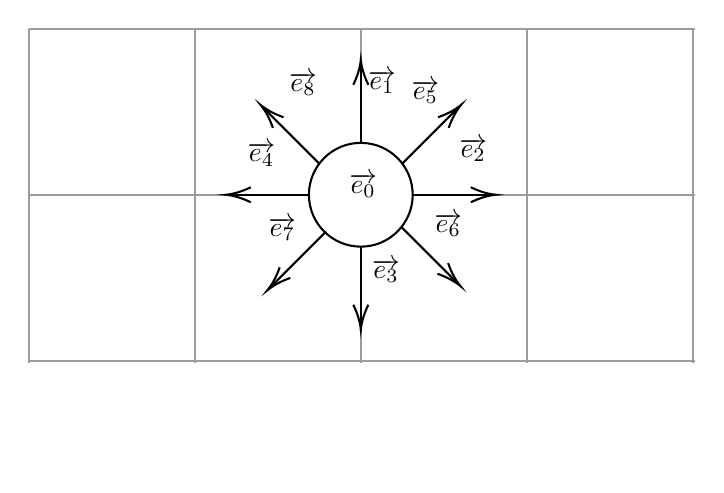
\begin{tikzpicture}[x=0.75pt,y=0.75pt,yscale=-1,xscale=1]
    %uncomment if require: \path (0,300); %set diagram left start at 0, and has height of 300

    %Straight Lines [id:da8888780735517332]
    \draw    (373.87,278.53) ;
    %Shape: Grid [id:dp03877998282701478]
    \draw  [draw opacity=0] (190,69) -- (511,69) -- (511,230) -- (190,230) -- cycle ; \draw  [color={rgb, 255:red, 155; green, 155; blue, 155 }  ,draw opacity=1 ] (190,69) -- (190,230)(270,69) -- (270,230)(350,69) -- (350,230)(430,69) -- (430,230)(510,69) -- (510,230) ; \draw  [color={rgb, 255:red, 155; green, 155; blue, 155 }  ,draw opacity=1 ] (190,69) -- (511,69)(190,149) -- (511,149)(190,229) -- (511,229) ; \draw  [color={rgb, 255:red, 155; green, 155; blue, 155 }  ,draw opacity=1 ]  ;
    %Shape: Circle [id:dp5022874038415199]
    \draw  [fill={rgb, 255:red, 255; green, 255; blue, 255 }  ,fill opacity=1 ] (325,149) .. controls (325,135.19) and (336.19,124) .. (350,124) .. controls (363.81,124) and (375,135.19) .. (375,149) .. controls (375,162.81) and (363.81,174) .. (350,174) .. controls (336.19,174) and (325,162.81) .. (325,149) -- cycle ;
    %Straight Lines [id:da04736893300326139]
    \draw    (350,174) -- (350,212) ;
    \draw [shift={(350,214)}, rotate = 270] [color={rgb, 255:red, 0; green, 0; blue, 0 }  ][line width=0.75]    (12.02,-3.62) .. controls (7.65,-1.54) and (3.64,-0.33) .. (0,0) .. controls (3.64,0.33) and (7.65,1.54) .. (12.02,3.62)   ;
    %Shape: Boxed Line [id:dp021303205536981507]
    \draw    (325,149) -- (287,149) ;
    \draw [shift={(285,149)}, rotate = 360] [color={rgb, 255:red, 0; green, 0; blue, 0 }  ][line width=0.75]    (12.02,-3.62) .. controls (7.65,-1.54) and (3.64,-0.33) .. (0,0) .. controls (3.64,0.33) and (7.65,1.54) .. (12.02,3.62)   ;
    %Shape: Boxed Line [id:dp539113257220927]
    \draw    (350,124) -- (350,86) ;
    \draw [shift={(350,84)}, rotate = 90] [color={rgb, 255:red, 0; green, 0; blue, 0 }  ][line width=0.75]    (12.02,-3.62) .. controls (7.65,-1.54) and (3.64,-0.33) .. (0,0) .. controls (3.64,0.33) and (7.65,1.54) .. (12.02,3.62)   ;
    %Shape: Boxed Line [id:dp44341141245264937]
    \draw    (375,149) -- (413,149) ;
    \draw [shift={(415,149)}, rotate = 180] [color={rgb, 255:red, 0; green, 0; blue, 0 }  ][line width=0.75]    (12.02,-3.62) .. controls (7.65,-1.54) and (3.64,-0.33) .. (0,0) .. controls (3.64,0.33) and (7.65,1.54) .. (12.02,3.62)   ;
    %Shape: Boxed Line [id:dp5984779454881499]
    \draw    (333.28,166.72) -- (306.41,193.59) ;
    \draw [shift={(305,195)}, rotate = 315] [color={rgb, 255:red, 0; green, 0; blue, 0 }  ][line width=0.75]    (12.02,-3.62) .. controls (7.65,-1.54) and (3.64,-0.33) .. (0,0) .. controls (3.64,0.33) and (7.65,1.54) .. (12.02,3.62)   ;
    %Shape: Boxed Line [id:dp16339365265718486]
    \draw    (330,134) -- (303.13,107.13) ;
    \draw [shift={(301.72,105.72)}, rotate = 45] [color={rgb, 255:red, 0; green, 0; blue, 0 }  ][line width=0.75]    (12.02,-3.62) .. controls (7.65,-1.54) and (3.64,-0.33) .. (0,0) .. controls (3.64,0.33) and (7.65,1.54) .. (12.02,3.62)   ;
    %Shape: Boxed Line [id:dp21948780896625064]
    \draw    (370,134) -- (396.87,107.13) ;
    \draw [shift={(398.28,105.72)}, rotate = 135] [color={rgb, 255:red, 0; green, 0; blue, 0 }  ][line width=0.75]    (12.02,-3.62) .. controls (7.65,-1.54) and (3.64,-0.33) .. (0,0) .. controls (3.64,0.33) and (7.65,1.54) .. (12.02,3.62)   ;
    %Shape: Boxed Line [id:dp05711106860687787]
    \draw    (369.72,164.72) -- (396.59,191.59) ;
    \draw [shift={(398,193)}, rotate = 225] [color={rgb, 255:red, 0; green, 0; blue, 0 }  ][line width=0.75]    (12.02,-3.62) .. controls (7.65,-1.54) and (3.64,-0.33) .. (0,0) .. controls (3.64,0.33) and (7.65,1.54) .. (12.02,3.62)   ;

    % Text Node
    \draw (343,137.4) node [anchor=north west][inner sep=0.75pt]    {$\overrightarrow{e_{0}}$};
    % Text Node
    \draw (352,87.4) node [anchor=north west][inner sep=0.75pt]    {$\overrightarrow{e_{1}}$};
    % Text Node
    \draw (396,120.4) node [anchor=north west][inner sep=0.75pt]    {$\overrightarrow{e_{2}}$};
    % Text Node
    \draw (354,178.4) node [anchor=north west][inner sep=0.75pt]    {$\overrightarrow{e_{3}}$};
    % Text Node
    \draw (294,122.4) node [anchor=north west][inner sep=0.75pt]    {$\overrightarrow{e_{4}}$};
    % Text Node
    \draw (373,92.4) node [anchor=north west][inner sep=0.75pt]    {$\overrightarrow{e_{5}}$};
    % Text Node
    \draw (384,156.4) node [anchor=north west][inner sep=0.75pt]    {$\overrightarrow{e_{6}}$};
    % Text Node
    \draw (304,158.4) node [anchor=north west][inner sep=0.75pt]    {$\overrightarrow{e_{7}}$};
    % Text Node
    \draw (314,88.4) node [anchor=north west][inner sep=0.75pt]    {$\overrightarrow{e_{8}}$};


    \end{tikzpicture}

\caption{D2Q9: 2D lattice with 9 discrete velocities.}
\label{fig:disc}
\end{figure}

There are two main steps in an iteration of an LBM:
\begin{enumerate}
    \item \textbf{Collision} - particles on each lattice site collide and redistribute along the discrete directions. Different collision operators can be used to model different behaviors.
    \item \textbf{Streaming} - particles move to neighboring lattice sites according to their velocity.
\end{enumerate}
Despite being developed from a mesoscale perspective, LBMs can be used for large flows as well \cite{sharma2020current}.

Lastly, microscopic scale flows and interactions are often modeled by individual particles obeying Newton's laws. The most common method for this is the Molecular Dynamics (MD) method \cite{koplik1989molecular}.
Generally these are less associated with CFD and seldom mentioned in the surrounding discussions, excluding specialized contexts.
I will not discuss them further in this thesis but they are nonetheless an interesting subject.

All things considered, we can identify two main categories of classical CFD methods:
\begin{itemize}
    \item \textbf{Continuum methods} - which numerically solve the partial differential equations governing the system (usually Navier-Stokes).
    \item \textbf{Lattice methods} - which model fluids as collections of fictitious particles moving on a lattice.
\end{itemize}

\section{Quantum Computing Fundamentals}
\label{sec:qc-basics}

Classical computing, when stripped of all abstraction and boiled down to its purest form is just applying specific operations (gates) on units of information (bits).
A chain of gates is called a Circuit or Algorithm, depending on the context.

While the fundamental principles involved are vastly different, Quantum Computing, in particular the Quantum Circuit formalism, mirrors this paradigm.

\paragraph*{The Qubit}
is the quantum counterpart for the bit, as the name suggests. Abstracting away the physical ways they are implemented, a qubit can store a binary value: 0 or 1.
Qubits are written using \emph{bra-ket} notation: $\ket{0}$, $\ket{1}$ for specific values or $\ket{x}$, $\ket{i}$, etc. for variables.
Unlike a bit which is a scalar, a qubit is actually a vector, with 
\begin{equation*}
  \ket{0} = \begin{pmatrix} 1 \\ 0 \end{pmatrix} \text{and} \ket{1} = \begin{pmatrix} 0 \\ 1 \end{pmatrix}
\end{equation*}
forming a \emph{basis}, known as the \emph{Computational Basis}.

It then follows that a qubit is not limited to the two basis states; in fact it can be any linear combination, as long as the qubit is \emph{normalized}.
When that happens, we say the qubit is in \emph{superpositon}.
For example: $\frac{1}{\sqrt2}\ket{0} + \frac{1}{\sqrt2}\ket{1}$ and $\frac{1}{\sqrt2}\ket{0} - \frac{1}{\sqrt2}\ket{1}$ are both equal superpositions of the computational basis states.
They are so important they get shorthand notation: $\ket{+}$ and $\ket{-}$ respectively. These two states form the \emph{Hadamard basis}.

Moreover, the coefficients are not restricted to real numbers: $\frac{1}{\sqrt2}\ket{0} + \frac{i}{\sqrt2}\ket{1}$ and $\frac{1}{\sqrt2}\ket{0} - \frac{i}{\sqrt2}\ket{1}$
are yet again important states: $\ket{+i}$ (or simply $\ket{i})$ and $\ket{-i}$ (not to be confused with $-\ket{i}$)

A register of multiple qubits is normally described by the \emph{tensor product} of the individual qubits.
\begin{equation*}
    \ket{0}\ket{+} = \ket{0} \otimes \ket{+} = \ket{0} \otimes (\frac{1}{\sqrt2}\ket{0} + \frac{1}{\sqrt2}\ket{1}) = \frac{1}{\sqrt2}\ket{00} + \frac{1}{\sqrt2}\ket{01}
\end{equation*}
Note, for products of computational basis states, notation is usually shortened: $\ket{0}\ket{0} = \ket{00}$

When moving to systems of multiple qubits, the representation power of the qubit becomes more apparent.
A register of 3 bits can represent 1 of 8 distinct values, but a register of 3 qubits represents stores up to 8 complex coefficients at once.

\paragraph*{Quantum Gates}
are what is applied to qubits in order to change their states and perform computation.
While there is only one single-bit classical gate ($\text{NOT}$; excluding the no-op gate), there are infinite single-qubit quantum gates.
Since qubits are vectors, naturally quantum gates end up being described by linear transformations (matrices) and applying a gate to a qubit is equivalent to matrix-vector multiplication.
The only restriction is that these quantum gates must be \emph{unitary}, in order to keep the qubits normalized. As a side effect this also means quantum gates are always invertible,
the inverse of a quantum gate being its conjugate transpose: $MM^{\dagger} = M^{\dagger}M = I$

\begin{equation*}
    H\ket{0} = \begin{pmatrix} \frac{1}{\sqrt{2}}  & \frac{1}{\sqrt{2}}  \\ \frac{1}{\sqrt{2}}  & -\frac{1}{\sqrt{2}}  \end{pmatrix} \begin{pmatrix} 1 \\ 0 \end{pmatrix} = \begin{pmatrix} \frac{1}{\sqrt{2}} \\ \frac{1}{\sqrt{2}} \end{pmatrix} = \ket{+}
\end{equation*}
This $H$ gate is known as the \emph{Hadamard Gate}, useful for creating equal superpositions of the basis states.

Another common gate is the quantum equivalent to the $\text{NOT}$ gate: $X$ gate and it functions accordingly: $X\ket{0} = \ket{1}$ and $X\ket{1} = \ket{0}$ (An alternative description to the full matrix is defining what the gate does to the computational basis states)
The interesting behavior comes from the fact that quantum gates are linear transformations, which means they distribute over addition and scalar multiplication.

\begin{equation*}
    X(\frac{1}{\sqrt3}\ket{0} + \frac{\sqrt2}{\sqrt3}\ket{1}) = \frac{1}{\sqrt3}X\ket{0} + \frac{\sqrt2}{\sqrt3}X\ket{1} = \frac{1}{\sqrt3}\ket{1} + \frac{\sqrt2}{\sqrt3}\ket{0}
\end{equation*}
This application of a quantum gate over an entire superposition is known as \emph{quantum parallelism}.

We can also have multiple-qubit gates describing operations impossible to decompose into single qubit gates.
Consider this gate
\begin{equation*}
    \text{CNOT} = \begin{pmatrix} 
1 & 0 & 0 & 0 \\ 
0 & 1 & 0 & 0 \\ 
0 & 0 & 0 & 1 \\ 
0 & 0 & 1 & 0 
\end{pmatrix}
\end{equation*}

It is described by the following transformations to the 2-qubit computational basis states:
\begin{equation*}
    \begin{aligned}
    \text{CNOT} \ket{00} &= \ket{00} \\
    \text{CNOT} \ket{01} &= \ket{01} \\
    \text{CNOT} \ket{10} &= \ket{11} \\
    \text{CNOT} \ket{11} &= \ket{10}
\end{aligned}
\end{equation*}
This is the \emph{Conditional-NOT gate}, negating the second qubit if and only if the first is $ket{1}$.
The first qubit is called the \emph{control} with the second being the \emph{target}
This pattern is common and many single qubit gates have \emph{controlled} versions.

Now observe what happens when the control qubit is in a superposition:
\begin{equation*}
    \text{CNOT}\ket{+}\ket{0} = \text{CNOT}(\frac{1}{\sqrt2}\ket{00} + \frac{1}{\sqrt2}\ket{10}) = \frac{1}{\sqrt2}(\text{CNOT}\ket{00} + \text{CNOT}\ket{10}) = \frac{1}{\sqrt2}(\ket{00} + \ket{11})
\end{equation*}
The resulting state, $\frac{1}{\sqrt2}(\ket{00} + \ket{11})$, cannot be decomposed as the tensor product of two individual qubits.
The values of the two qubits became linked, they are no longer independent. This is known as \emph{entanglement} and is another cornerstone of quantum computing. 

\paragraph*{Measurement}
is the one concept that does not exactly have a classical analogue, but is integral for quantum computing.
Despite qubits "storing" more information, that information is not directly accessible.
To read the value of a qubit, a \emph{measurement} must be performed, and the result is always a basis state.

When measuring a qubit that is in a superposition, one of the basis states is obtained at random.
The probability of obtaining a specific state is equal to the amplitude squared of the state's coefficient the qubit. This is known as the \emph{Born Rule}
For example the state $\frac{1}{\sqrt3}\ket{0} + \frac{\sqrt2}{\sqrt3}\ket{1}$ has a $\frac{1}{3}$ chance of yielding $\ket{0}$, with the rest being $\ket{1}$.
This is why qubits had the restriction of being normalized, because the sum of measurement probabilities must equal 1.

The choice of measurement basis is arbitrary and dictates whether something even is a superposition or not.
Measuring $\ket{+}$ in the computational basis yields equal probability outcomes, yet measuring in the Hadamard basis always gives the same answer, since $\ket{+}$ is a part of that basis.

This limitation is what makes designing meaningful quantum algorithms challenging. 
It might seem like it completely negates the previous upsides, but clever manipulation of the quantum states can still lead to faster algorithms in terms of computational complexity.
Famous examples include Simon's Algorithm, Grover's Algorithm and Shor's Algorithm \todo{citations here}.

\todo{add citations}
\section{Linear Combination of Unitaries}
\label{sec:lcu}

As previously discussed, non-unitary matrices cannot be quantum gates.
This significantly limits the



\todo{REVISION: add complexity analysis to section 2.3 (Quantum Approaches to CFD)}
\section{Quantum Approaches to CFD}
\label{sec:qcfd}

Some of the earliest work in quantum algorithms for CFD was done by Yepez in the late 90s to early 2000s.
He showed that the \emph{Quantum Lattice Gas Automata} (QLGA), which had been developed for quantum multi-body problems \cite{boghosian1997gas}, could be used to model classical fluid flows \cite{yepez1998lattice}.
He later proposed an algorithm for the QLGA on a Type-II Quantum Computer, which is a hybrid system of quantum computers that can communicate via classical channels. \cite{yepez2001lattice}.

After these initial developments, there was a long period of little to no activity in the field.
During this time, however, several important quantum algorithms were developed, such as the HHL algorithm for solving linear systems of equations \cite{harrow2009quantum} or various ordinary differential equations (ODE) solvers \cite{kacewicz2006almost,leyton2008quantum}.

Starting in 2020, the field of quantum computational fluid dynamics has seen a bit of a resurgence.
Unlike the early work, newer research was more focused on using the aforementioned quantum algorithms to more efficiently solve the Navier-Stokes equations \cite{gaitan2020finding, jaksch2023variational}.
The QLGA was not abandoned, however, and like its classical counterpart it evolved into the \emph{Quantum Lattice Boltzmann Method} (QLBM) \cite{budinski2021quantum, itani2024quantum}.

Mirroring the classical approaches, quantum algorithms for CFD also fall under the two categories of continuum and lattice methods.
Subsequently, I will discuss a couple of quantum algorithms for CFD, focusing on the ones most representative of their category.

\paragraph*{Quantum Navier-Stokes Solver}
In 2020 Gaitan published a quantum algorithm for solving the Navier-Stokes equations \cite{gaitan2020finding}.
Despite being presented in the context of CFD, the author claims it has general applicability to any system of partial differential equations.
The algorithm itself consists of two main parts:
\begin{enumerate}
    \item Discretizing the PDEs to a set of ODEs. Gaitan uses the Finite Difference Method (FDM) and briefly discusses exploring other methods in future work.
    \item Solving the resulting ODEs using \emph{Kacewicz's quantum algorithm} \cite{kacewicz2006almost}. The algorithm is claimed to be almost optimal.
\end{enumerate}
Kacewicz's ODE algorithm is a hybrid algorithm that makes use of the \emph{Quantum Amplitude Estimation Algorithm} \cite{brassard2002quantum} to achieve a speedup over classical methods.

To validate the algorithm, Gaitan uses it to simulate an inviscid compressible 1D flow through a convergent-divergent nozzle
The simulations were performed using Qiskit \cite{qiskit2024} and showed great agreement with the exact analytical solution.

To determine the performance gain, Gaitan performs a complexity analysis of the algorithm compared with both deterministic and random classical algorithms.
The results show that the time complexity depends on the smoothness (Hölder class) of the function being solved. For smooth functions, all algorithms have the same complexity.
For "rough" functions, however, the quantum algorithm shows a square root speedup over probabilistic classical algorithms and an exponential speedup over deterministic classical algorithms.

The main drawback of the algorithm is the fact that it is hybrid. In particular it repeatedly uses the Quantum Amplitude Estimation Algorithm as a subroutine. The constant communication between the quantum and classical parts of the algorithm could be a bottleneck in practice.

\paragraph*{Hydrodynamic Schrödinger Equation}
While the vast majority of continuum methods are focused on the Navier-Stokes equations, they are not the only option available.
In 2023, Yang and Meng proposed a model for fluid flows based on the \emph{Schrödinger equation} \cite{meng2023quantum}.

The \emph{Madelung equations} are a set of equations that serve as an alternate formulation of the Schrödinger equation written in hydrodynamical form \cite{schonberg1954hydrodynamical}.
The key idea behind this formulation is the similarity between some quantities of quantum and fluid mechanics.
\begin{table}[ht!]
    \caption{Similarities between quantum and fluid quantities.}
    \label{tab:quantities}
    \centering
    \begin{tabular}{|c|c|c|}
    \hline
    & $\rho$ & $\pmb{J}=\rho \pmb{u}$ \\
    \hline
    Quantum Mechanics & Probability Density & Probability Current \\
    \hline
    Fluid Mechanics & Mass Density & Momentum \\
    \hline
    \end{tabular}
\end{table}

Since it is formulated in terms of hydrodynamical variables, we can imagine a fictitious fluid that obeys these equations. Because the Madelung equations are equivalent to the Schrödinger equation, they can more naturally be implemented on a quantum computer.

The major problem, however, is that this fictitious fluid does not behave similarly enough to real fluids. In particular it lacks viscosity and vorticity.
This is where Yang and Meng's contribution lies. They managed to generalize the Madelung equations to better model real fluids.
They called the flow described by this equation the \emph{Schrödinger Flow}.
The authors validated that the Schrödinger Flow can indeed model real fluids by using it to simulate turbulent flows in 2D and 3D. The simulation was a Direct Numerical Simulation (DNS) done classically.

Alongside the new equations, they also proposed a fully quantum algorithm for simulating the case of the Incompressible Schrödinger Flow.
The algorithm consists of 5 steps per time step of simulation, with measurements only at the end of the simulation.

The algorithm was tested by simulating a 1D steady flow and a 2D turbulent flow.
The simulations were performed using Qiskit \cite{qiskit2024} and matched the theoretical predictions.

Unfortunately, the algorithm does not yet provide a speedup over classical methods. Of the 4 steps in the algorithm, steps 2 and 4 are bottlenecks with no known efficient implementations.
Steps 1 and 3 do provide exponential speedups over classical implementations of those specific operations.
The authors want to tackle these bottlenecks in future works.

Even ignoring the proposed algorithm's current limitations, the Schrödinger Flow model itself is not perfect.
Despite being able to model some turbulent flows it is not yet a universal model for all fluid flows.

\paragraph*{Quantum Lattice Boltzmann Methods}
In the classical Lattice Boltzmann Method, we discretize space and velocity and try to model the \emph{fluid density}.
The function $f_{i}(x,t)$ denotes the "amount" of fluid moving in direction $i$ at position $x$ and time $t$.
Unsurprisingly, summing over $i$ gives the fluid density at lattice site $x$ and time $t$.
There is however an alternative way to interpret this function, one that better leads to \emph{Quantum Lattice Boltzmann Methods} (QLBMs).

Instead of thinking about many particles moving in different directions, we can imagine a single particle that has different \emph{probabilities} of moving in different directions.
Now our particle is in a \emph{superposition} of the different directions. We can model a single lattice site as a quantum state:
\begin{displaymath}
    \label{eq:qlbm}
    \ket{\psi_x} = \ket{x}\sum_{i} \frac{f_{i}(x)}{f(x)} \ket{i}
\end{displaymath}
where $\ket{x}$ is an encoding of the site x and $\ket{i}$ is the basis state corresponding to direction $i$.

An alternative mapping is to consider a tensor product instead of a sum:
\begin{displaymath}
    \label{eq:qlbm2}
    \ket{\psi_x} = \ket{x}\bigotimes_{i} (\sqrt{1-f_i(x)}\ket{0} + \sqrt{f_i(x)}\ket{1})
\end{displaymath}

In both cases the total state is a superposition of all lattice sites.
Unfortunately, Schalkers and Möller showed that both of these encodings have issues \cite{schalkers2024importance}:
\begin{itemize}
    \item The first encoding does not admit a unitary \emph{collision operator}
    \item The second encoding does not admit a unitary \emph{streaming operator}
\end{itemize}

This means that any practical QLBM will have to use more sophisticated encodings, techniques or trade-offs.

There are many different QLBMs proposed, each with different encodings and ways to implement the collision and streaming operators.
I will be focusing on Budinski's QLBM \cite{budinski2021quantum} because of its intuitive encoding and importance in literature.
Other QLBMs will be briefly mentioned when relevant.

Given a D1Q2 lattice with $M$ sites, Budinski's encoding is:
\begin{displaymath}
    \label{eq:qlbm3}
    \ket{\psi} = \ket{0} \sum_{i=0}^{2M-1} \frac{f_{\alpha, i}}{||f||}\ket{i}
\end{displaymath}
where $\alpha$ is $1$ or $2$ for the two different velocities and $i$ is the lattice site.
The encoding can be generalized to other lattice schemas.

This encoding looks similar to the first encoding presented, but the auxiliary qubit is very important.
That qubit allows Budinski to implement the normally non-unitary collision operator as a \textbf{block encoding}\footnote{A block encoding is a way to embed a non-unitary matrix into a larger unitary matrix.}.

The propagation step is implemented similar to a \textbf{Quantum Walk} \cite{childs2009universal}, by shifting the qubits left and right respectively.

Budinski tested his QLBM by simulating a simple diffusion using both D1Q2 and D2Q5 lattices.
The results match both analytical solutions and classical simulations.

For a DmQn lattice with M sites, the complexity analysis of this algorithm shows it is logarithmic in the number of lattice sites: $O(n\log(mM))$. This is a significant speedup over classical Lattice Boltzmann Methods which are linear.
Unfortunately this QLBM has a crucial limitation: each time step requires measurements and a new initialization of the state.
It is especially oppressive as the encoding (which was excluded from the above complexity) is linear in the number of lattice sites.

There are more recent developments that try to solve these problems.
For instance, Kocherla et al. proposed a QLBM that can delay the need for measurements until the end of the simulation \cite{kocherla2024fully}.

\todo{REVISION: merge section 2.4 (Advection-Diffusion QLBM) into section 2.3 (Quantum Approaches to CFD)}
\section{The Advection-Diffusion QLBM}
\label{sec:qlbm-detail}

The QLBM, as the name suggests, is the quantum version of the classical Lattice Boltzmann Method (LBM) algorithm.

LBMs work by discretizing space into a lattice structure, where each lattice site contains a set of \textbf{link distributions}.
Each link distribution has an associated link velocity and represents the proportion of the simulated quantity that will propagate along that link.
Discretization schemes are named after the number of dimensions and the number of links: D1Q3 for 1D with 3 links, D2Q9 for 2D with 9 links, D3Q27 for 3D with 27 links.

An iteration of the algorithm consists of two main steps:
\begin{enumerate}
    \item \textbf{Collision:} The values of the link distributions are updated based on a \textbf{collision operator}. The specific operator depends on details of the simulated behavior.
    \item \textbf{Streaming:} The distribution values are propagated to neighboring sites based on the defined link velocities.
\end{enumerate}

Finally, the link distributions are summed up in order to recover the macroscopic distribution.

One of the earliest implementations of a QLBM was proposed by Budinski \cite{budinski2021quantum}.
He proposed a quantum circuit that could simulate flows governed by the \textbf{advection-diffusion equation}:

\begin{equation}
    \partial_t\Phi = D\nabla^{2}\Phi - \nabla(\mathbf{u}\Phi)
\end{equation}

Where $\Phi(x)$ is the distribution function, $D$ is the diffusion coefficient and $\mathbf{u(x)}$ is the velocity field.

He later extended the method to the Navier-Stokes equations \cite{ljubomir2022quantum} via the stream-vorticity formulation and validated his results in a lid-driven cavity flow simulation.

Unfortunately, this matrix is not unitary, but we can circumvent this by using a technique called \textbf{Linear Combination of Unitaries} \cite{childs2012hamiltonian}.
We can express $M$ as $\frac{1}{2}(U_1 + U_2)$ with $U_1 = M + i\sqrt{I - M^2}$ and $U_2 = M - i\sqrt{I - M^2}$.

These matrices are both unitary and can be implemented as quantum gates.

To apply the desired linear combination, we utilize an ancilla qubit prepared in the state $\ket{0} + \ket{1}$.
Then we apply each of the unitaries conditioned on the $\ket{0}$ and $\ket{1}$ states of the ancilla qubit, respectively.
Other than the ancilla, the drawback of this method is that our desired result is only present in the $\ket{0}$ substate.
This is not a problem when performing Statevector simulations, but it increases the number of shots required for running the algorithm on a real quantum computer.
